
\documentclass[11pt,letterpaper]{article}

% Load some basic packages that are useful to have
% and that should be part of any LaTeX installation.
%
% be able to include figures
\usepackage{graphicx}
% get nice colors
\usepackage{xcolor}

% change default font to Palatino (looks nicer!)
\usepackage[latin1]{inputenc}
\usepackage{mathpazo}
\usepackage[T1]{fontenc}
% load some useful math symbols/fonts
\usepackage{latexsym,amsfonts,amsmath,amssymb}

% comfort package to easily set margins
\usepackage[top=1in, bottom=1in, left=1in, right=1in]{geometry}

% control some spacings
%
% spacing after a paragraph
\setlength{\parskip}{.15cm}
% indentation at the top of a new paragraph
\setlength{\parindent}{0.0cm}


\begin{document}

\begin{center}
\Large
Ay190 -- Worksheet 12\\
Anthony Alvarez\\
Date: February 20, 2014
\end{center}

\section{Poisson Equation}

We will consider the Poisson equation.
$$ \nabla^2\Phi = 4\pi G\rho$$

\subsection{Reading Data}

First we read the data in and determine which columns are which. We determine
the first column is simply a count. Column 2 is the mass, 3 is the radius, 4 is
temerature, 5 is density, 6 is radial velocity, 7 is electron fraction and 8 is
rotational velocity (constant and 0 for a non rotating star). 

Next we make a plot of $\rho(r)$ as you can see in ~\ref{fig:rhor}. Note that 
we restirct our selves to $r < 10^9 cm$.

\begin{figure}[bth]
\centering
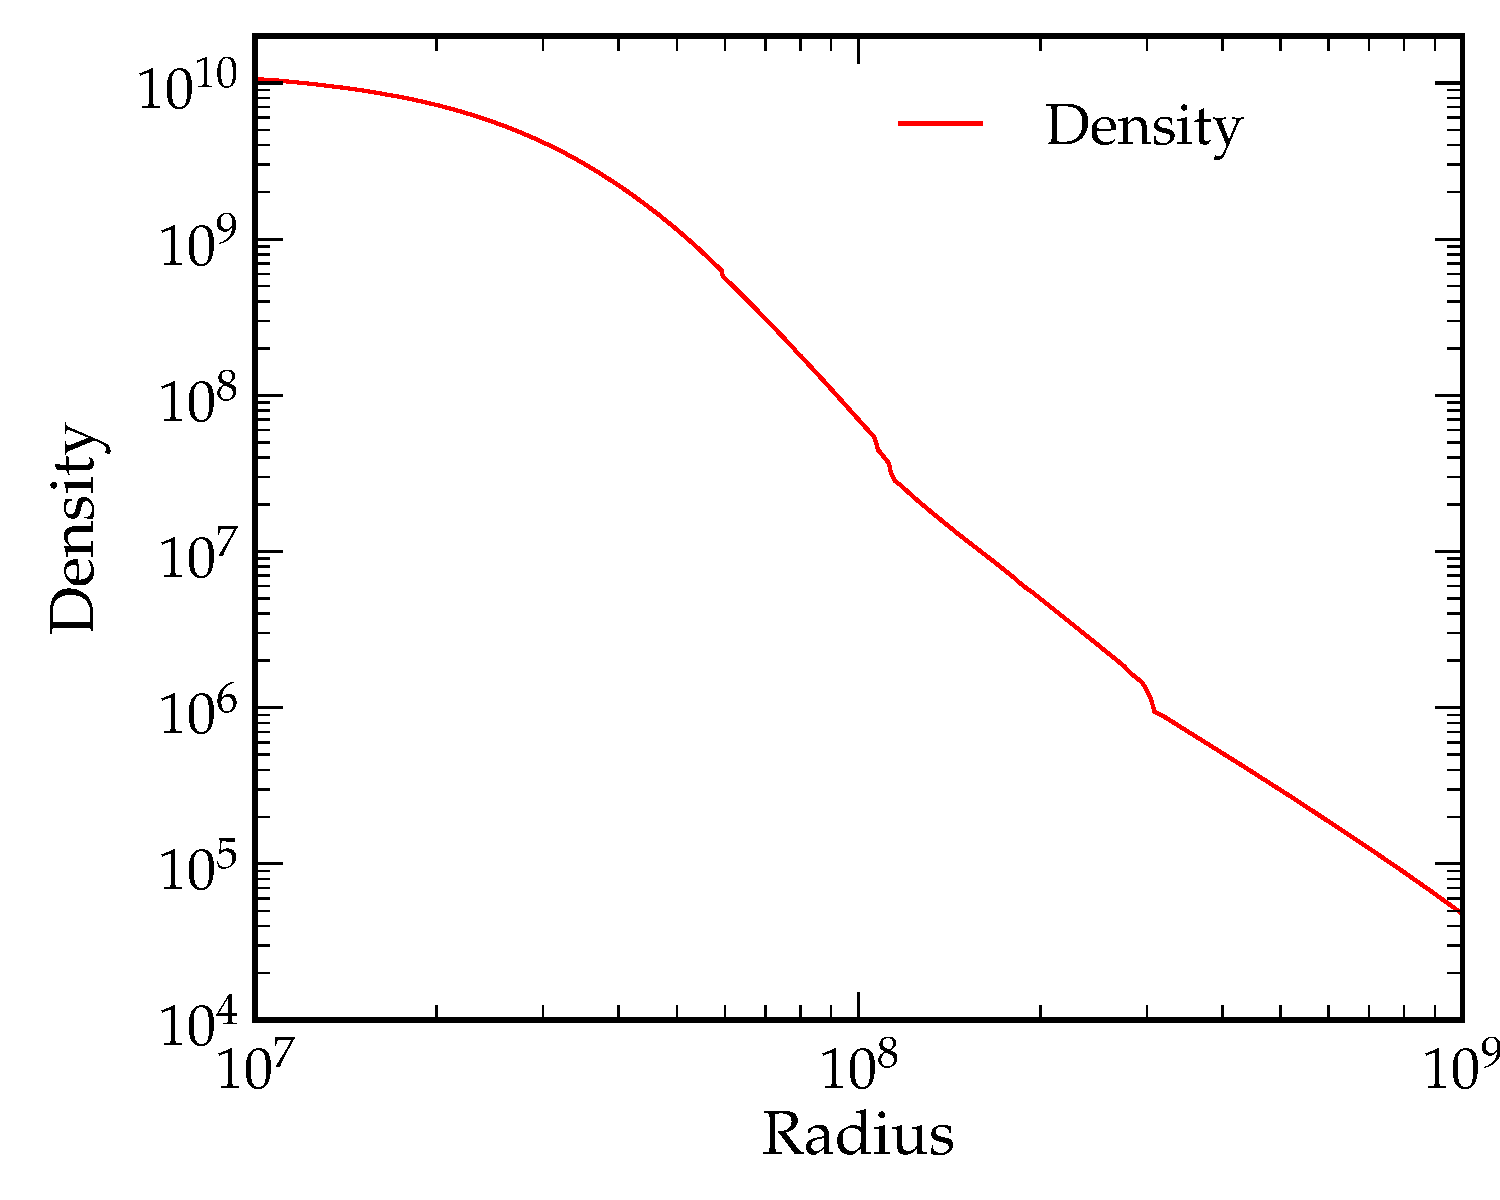
\includegraphics[width=0.5\textwidth]{1.pdf}
\caption{Plot of $\rho(r)$ for the inner part of the star. }
\label{fig:rhor}
\end{figure}

\subsection{Equidistant Grid}

We use linear interpolation to put the data onto an equidistant grid from
$10^7cm$ to $10^9cm$. We can see that this ~\ref{fig:rhor_interp} is very 
similar, if not indistinguishable from ~\ref{fig:rhor}. 

\begin{figure}[bth]
\centering
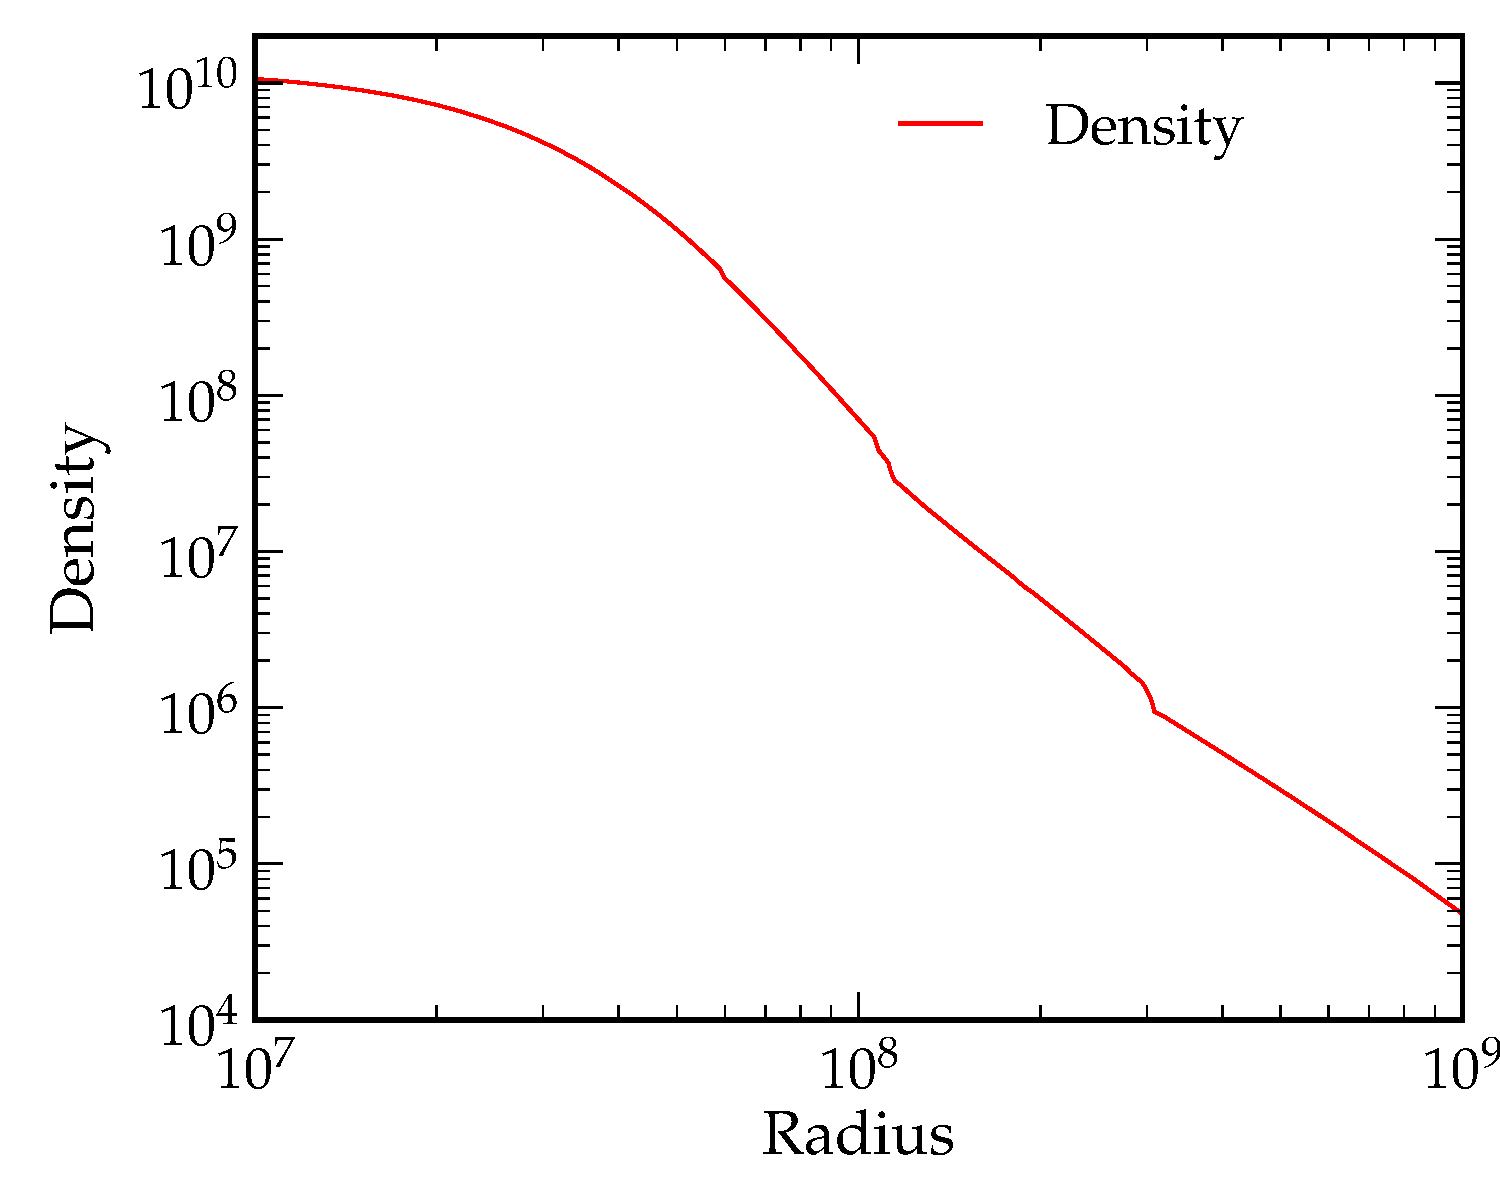
\includegraphics[width=0.5\textwidth]{2.pdf}
\caption{Plot of linearly interpolated $\rho(r)$ for the inner part of the star.}
\label{fig:rhor_interp}
\end{figure}.

\subsection{Constant Density $\Phi$}

First we decompose the Poisson equation into two coupled first order ODEs for
$\Phi$ and $\Phi' = u$. Then we use forward Euler integrator to find the value 
for $\Phi$ given the boundary conditions at $r=0$ are that $\Phi' = 0$ since 
there should be no gravitational force at the center of the star. 

Since poisson equation only determies $\Phi$ upto a constant we adjust the outer
boundary condition to match the known analytic $\Phi$ for a constant density. We
can see that there is good agreement between the analytic value and the forward
Euler integrated value in ~\ref{fig:phi_const_rho}. 

\begin{figure}[bth]
\centering
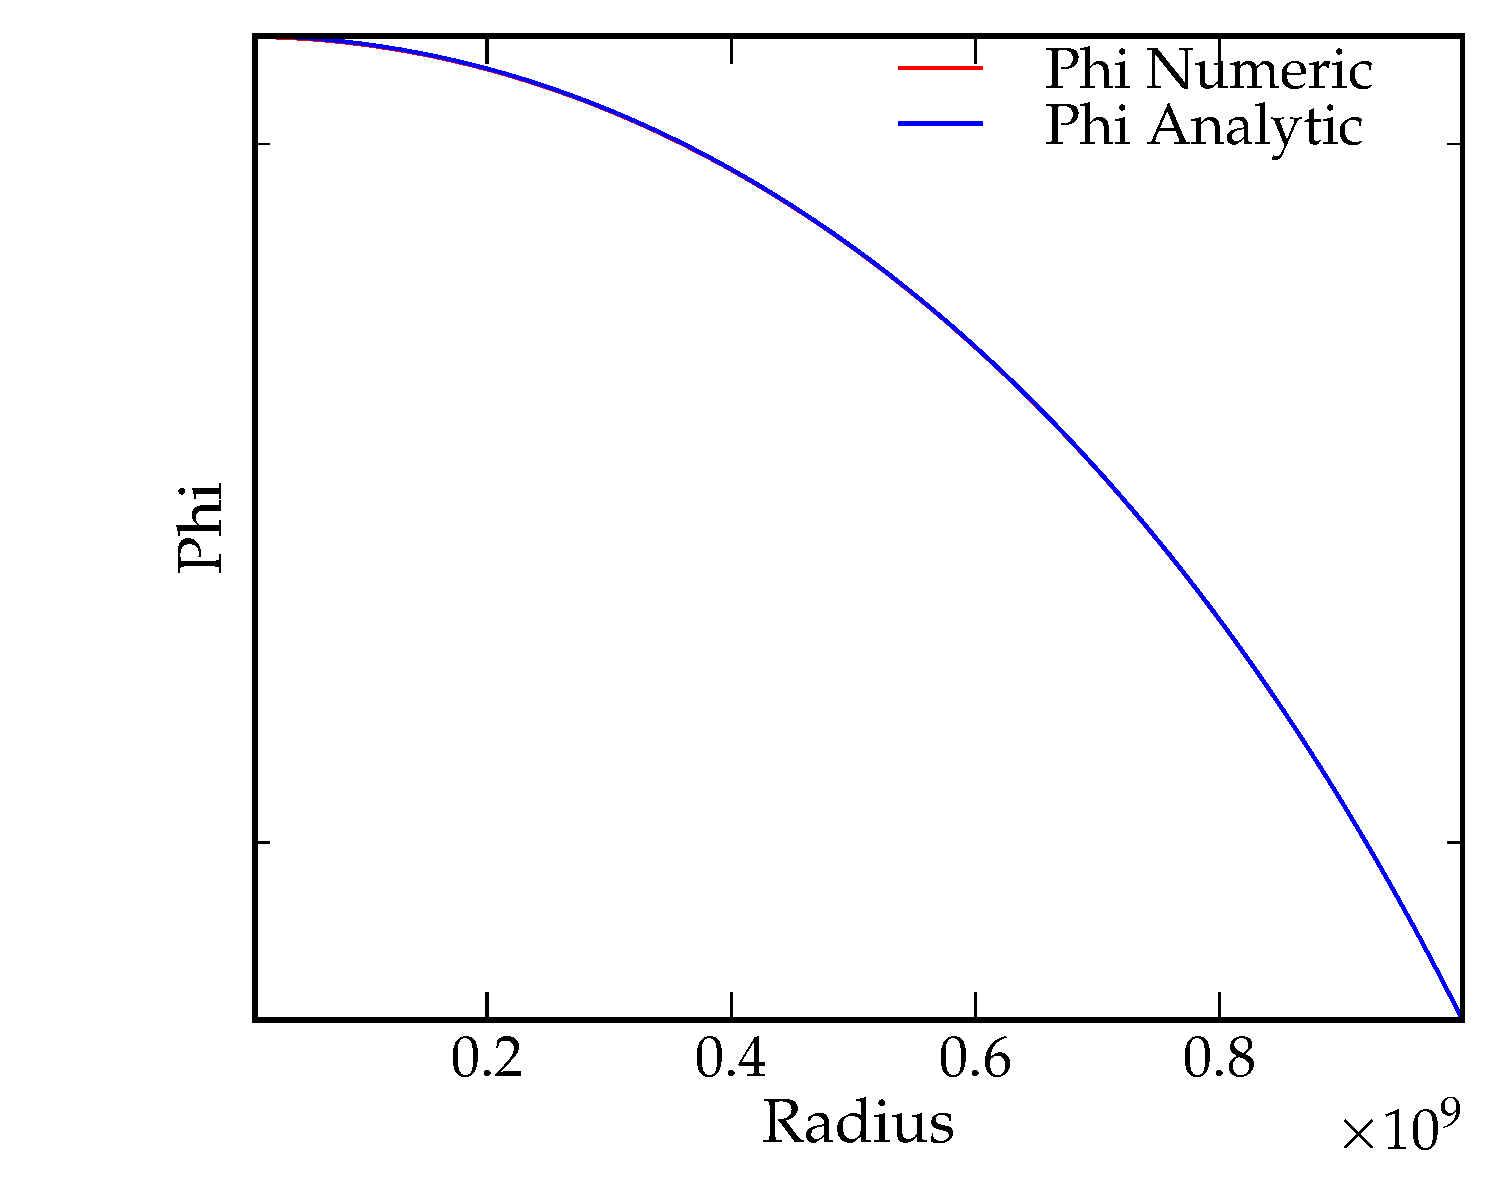
\includegraphics[width=0.5\textwidth]{3a.pdf}
\caption{$-\Phi$ for a cosntant density star. We graph -$\Phi$ to get it on a 
log plot.}
\label{fig:phi_const_rho}
\end{figure}

We also find that the convergance for the Forward Euler integrator is 1.00, just
like we would expect. With this confirmed we feel free to move on to the actual
supernova data. 

\subsection{Supernova Collapse $\Phi$}

Now that we have verified our forward Euler on a case where we know the analytic
answer we are able to implement it on a new problem. We see in ~\ref{fig:phi}
that the value of $\Phi(r= 10^9cm)$ rouhly converges to $5e18$ which makes sense.

\begin{figure}[bth]
\centering
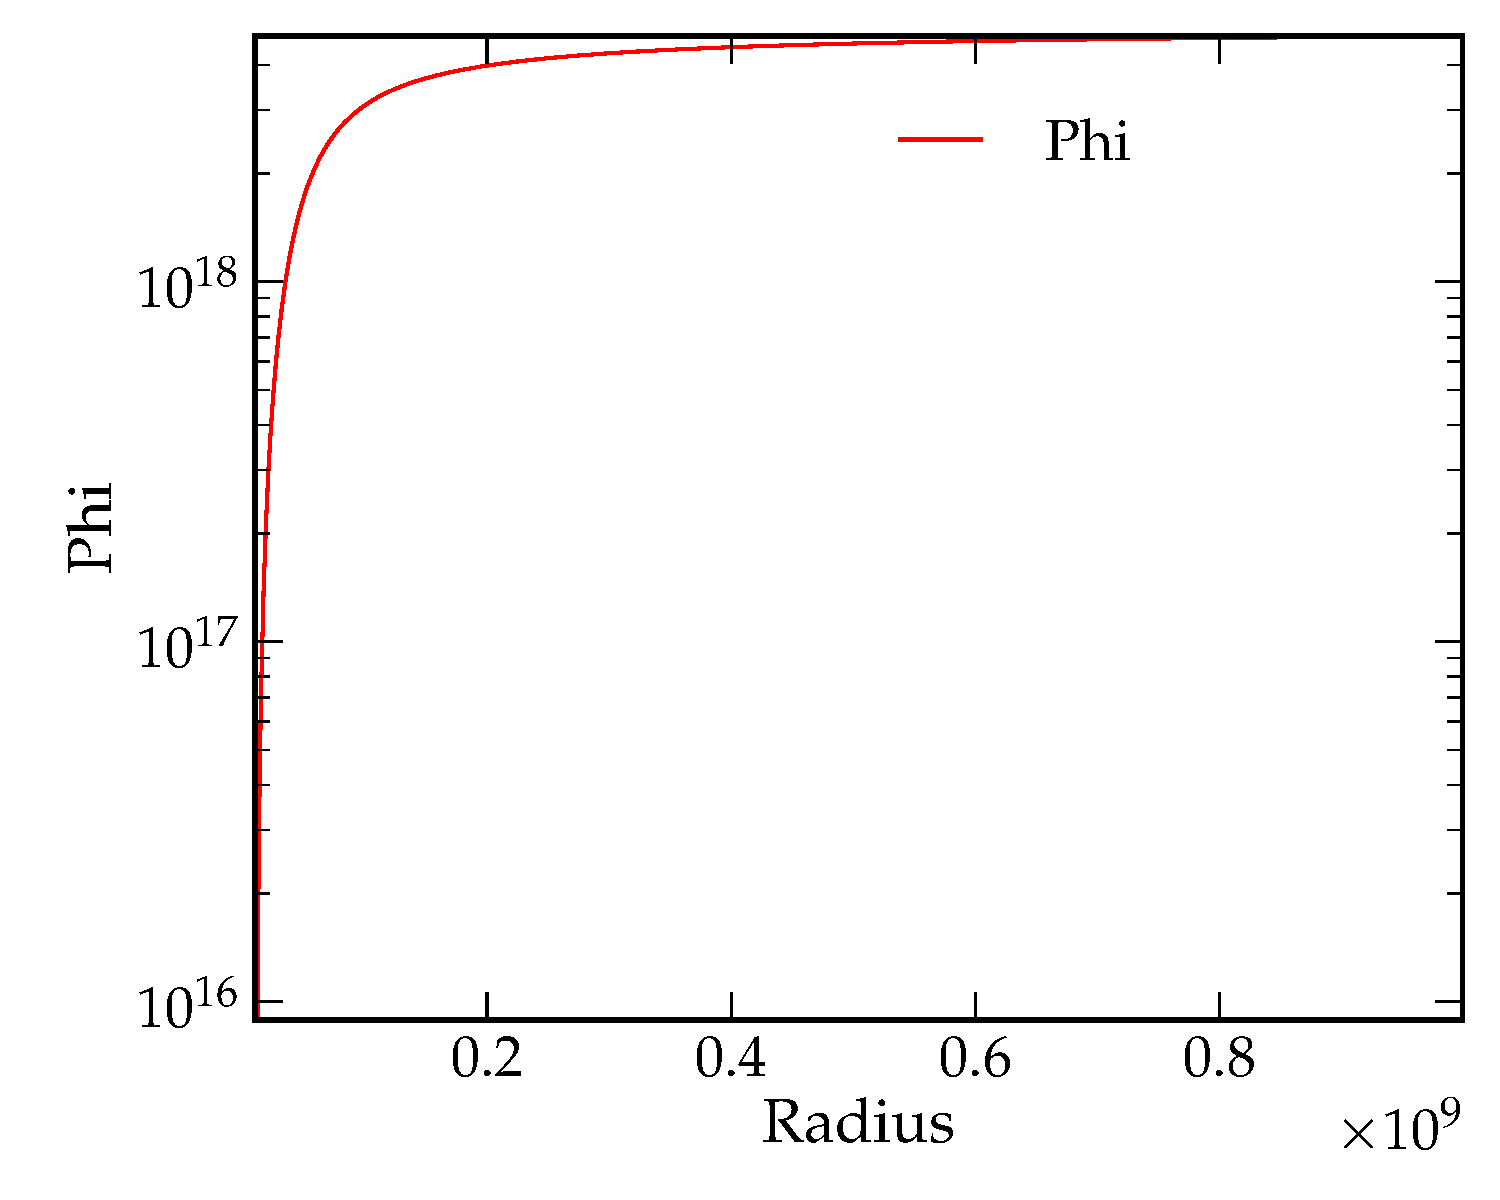
\includegraphics[width=0.5\textwidth]{3.pdf}
\caption{$-\Phi$ for a Supernova Colapse star. We graph -$\Phi$ to get it on a 
log plot.}
\label{fig:phi}
\end{figure}

\end{document}




